\clearpage

\lehead[]{\sf\hspace*{-2.00cm}\textcolor{white}{\colorbox{lightblue}{\parbox[c][0.70cm][b]{1.60cm}{
\makebox[1.60cm][r]{\thechapter}\\ \makebox[1.60cm][r]{ÜBUNG}}}}\hspace{0.17cm}\textcolor{lightblue}{\chaptertitle}}
\rohead[]{\textcolor{lightblue}{\chaptertitle}\sf\hspace*{0.17cm}\textcolor{white}{\colorbox{lightblue}{\parbox[c][0.70cm][b]{1.60cm}{\thechapter\\
ÜBUNG}}}\hspace{-2.00cm}}
%\chead[]{}
\rehead[]{\textcolor{lightblue}{AvHG, Inf, My}}
\lohead[]{\textcolor{lightblue}{AvHG, Inf, My}}

\section{Threads -- Übungen}

\subsection{Aufgabe 1: Rennendes Pferd}

Programmiere eine Animation, in der ein Pferd wiederholt von links nach rechts
über den Bildschirm galoppiert.

Erzeuge dazu ein neues Anwendungsfenster (in Eclipse: Rechtscklick auf das
Package im Package Explorer $\rightarrow$ \myPMI{New} $\rightarrow$ \myPMI{Other
\ldots} $\rightarrow$ \myPMI{Window Builder} $\rightarrow$ \myPMI{Swing
Designer} $\rightarrow$ \myPMI{JFrame}) und erzeuge eine Komponente
\lstinline|zeichenflaeche| (die du von \myClass{JPanel} ableitest). Lade im
Anwendungsfenster die beiden Bilder \myFile{horse1.gif} und \myFile{horse2.gif}.
Überschreibe die \lstinline|paintComponent()|-Methode von
\lstinline|zeichenflaeche|, und zeichne in dieser Methode das Pferd immer
abwechselnd einmal mit dem ersten und anschließend mit dem zweiten Bild.
Verschiebe außerdem die x-Position des Pferdes bei jedem Aufruf von
\lstinline|paintComponent()| um 10 Pixel nach rechts.


\begin{minipage}{0.6\textwidth}
Damit die \lstinline|paintComponent()| wiederholt aufgerufen wird, sollst du
eine zweite Klasse programmieren, die sich von der Klasse \myClass{Thread}
ableitet (benutze nicht \myClass{javax.swing.Timer}). Übergib der Klasse im
Konstruktor einen Verweis auf das Anwendungsfenster. Füge in der
\lstinline|run()|-Methode eine Endlosschleife ein, in der nach einer Wartezeit
von 100 Millisekunden immer wieder die \lstinline|repaint()|-Methode des
Anwendungsfensters aufgerufen wird.
\end{minipage}
\hfill
\begin{minipage}{0.25\textwidth}
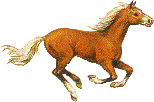
\includegraphics[width=1.0\textwidth]{./inf/SEKII/26_Java_Threads/Pferd.png}
\end{minipage}


\subsection{Aufgabe 2: Oldtimer}

Erstelle wie in der Abbildung ein Anwendungsfenster mit zwei Buttons und einer
Zeichenfläche, die von der Klasse \myClass{JPanel} abgeleitet wird.

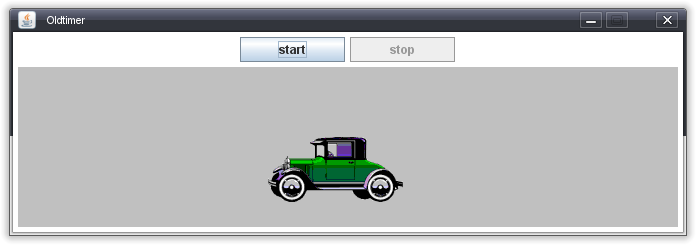
\includegraphics[width=1.0\textwidth]{./inf/SEKII/26_Java_Threads/Oldtimer.png}

Lade das Bild \myFile{car.gif} und zeichne es in der Mitte der Zeichenfläche.
Verschiebe die x-Position des Autos in der \lstinline|paintComponent()|-Methode
der Zeichenfläche bei jedem Aufruf ein Stück nach links, so dass das Auto
rollt, wenn ein Timer-Thread für ein regelmäßiges Neuzeichnen des Fensters
sorgt. Wenn das Auto links aus der Zeichenfläche herausgefahren ist, soll es
von rechts wieder in die Zeichenfläche hinein gleiten.

Zu Beginn soll jedoch noch kein Timer-Thread laufen und das Auto steht deshalb
still. Der Stopp-Button ist disabled. Wenn man auf den Start-Button drückt,
soll ein Timer-Thread gestartet werden. Dieser ruft in einer Schleife
wiederholt die \lstinline|repaint()|-Methode der Anwendung auf. Die Schleife des
Threads läuft so lange, bis eine boolesche Variable \lstinline|anhalten| auf
\lstinline|true| gesetzt wird. Dann beendet der Thread die Schleife und die
\lstinline|run()|-Methode und hört damit auf zu existieren. Wenn der Benutzer
auf den Stopp-Button drückt, wird die boolesche Variable auf \lstinline|true|
gesetzt, um dem Thread zu signalisieren, dass er seine Arbeit beenden soll.

Sorge dafür, dass der Stopp-Button immer dann disabled ist, wenn kein Thread
läuft, und der Start-Button disabled ist, wenn ein Thread am Laufen ist.


\subsection{Aufgabe 3: Jumping Potatoes}

Erstelle ein neues Anwendungsfenster mit einer Zeichenfläche mit einer Breite
von 900 Pixeln und einer Höhe von 350 Pixeln hat. Lade in dem Anwendungsfenster
das Bild \myFile{potato.gif}.

Programmiere außerdem eine Klasse \myClass{Potato}. Die Klasse besitzt als
Variablen das Anwendungsfenster und die x- und y-Position der Kartoffel (das
Bild muss die Klasse nicht kennen). Alle drei Werte werden im Konstruktor als
Parameter übergeben.

Erzeuge im Anwendungsfenster ein Array von zehn Potatoes. Alle Potatoes sollen
die y-Position 200 erhalten. Die x-Position des ersten Kartoffel soll bei 40
Pixel liegen. Die anderen Potatoes sollen jeweils im Abstand von 80 Pixel
folgen. Zeichne die Potatoes in der \lstinline|paintComponent()|-Methode der
Zeichenfläche, in dem du in einer Schleife zehn mal das Bild zeichnest. Die x-
und y-Position holst du dir dabei jeweils von dem \myClass{Potato}-Objekt mit
dem entsprechenden Index.

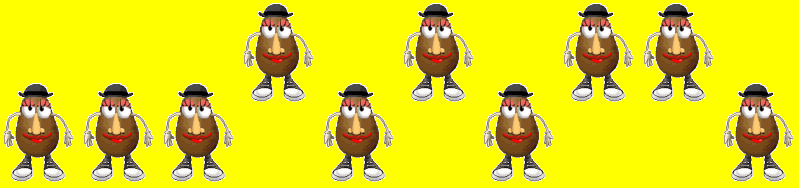
\includegraphics[width=1.0\textwidth]{./inf/SEKII/26_Java_Threads/JumpingPotatoes.png}

Leite die Klasse \myClass{Potato} nun von der Adapter-Klasse
\myClass{MouseAdapter} ab. Du musst dann lediglich die Methode
\lstinline|mouseClicked()| sinnvoll überschreiben. Registriere den
\myClass{MouseListener} auf die Komponente \lstinline|zeichenflaeche|. Wenn der
Benutzer mit der Maus in das Fenster klickt, prüft die Klasse, ob der Benutzer
auf das dem \myClass{Potato}-Objekt zugeordnete Bild geklickt hat (ein Bild
besitzt eine Breite von 74 Pixel und eine Höhe von 100 Pixel). Wenn die Potato
angeklickt wurde, soll sie nach oben springen. Falls der Benutzer die linke
Maustaste benutzt (\lstinline|MouseEvent.BUTTON1|), springt die Kartoffel 80
Pixel hoch. Falls der Benutzer die rechte Maustaste verwendet
(\lstinline|MouseEvent.BUTTON3|), springt die Kartoffel 160 Pixel hoch. Setze
dazu jeweils die y-Position geeignet um und veranlasse, dass das
Anwendungsfenster neu gezeichnet wird, damit der Benutzer den Sprung auch
sieht. Merke dir außerdem die ursprüngliche y-Position in einer globalen
Variablen, damit die Potato später wieder dahin zurückkehren kann.

Die Potato soll zwei Sekunden in der erhöhten Position bleiben und anschließend
automatisch wieder zurück springen. Erzeuge dazu einen Thread, der das Objekt
der angeklickten Kartoffel im Konstruktor als Parameter erhält. Der Thread muss
in der \lstinline|run()|-Methode nur einmal zwei Sekunden warten. Anschließend
ruft er eine Methode des \myClass{Potato}-Objekts auf, die die y-Position wieder
zurücksetzt und das Anwendungsfenster neu zeichnet.

Wenn du alles richtig programmiert hast, kann man mehrere Potatos nacheinander
anklicken, die dann zeitlich versetzt wieder in ihre Ausgangsposition
zurückspringen.


\subsection{Aufgabe 4: Störrischer Esel}

\begin{compactenum}[a)]
\item Erzeuge ein Anwendungsfenster mit einer Zeichenfläche mit einer Breite
von mindestens 600 Pixeln. Lade im Anwendungsfenster das Bild \myFile{esel.gif}.
Das Bild besitzt eine Breite von 140 und eine Höhe von 130 Pixel. Zeichne den
Esel zu Beginn ungefähr in der Mitte des Fensters.

\item Wenn man mit der Maus vor oder hinter den Esel klickt, soll der Esel
 weglaufen. Überprüfe dazu zunächst, ob sich die y-Position des Mausklicks im
 Bereich des Eselbildes befindet. Falls dies nicht der Fall ist, reagiert der
 Esel nicht. Falls sich die y-Position im Eselbereich befindet, weicht der Esel
 entweder nach links oder nach rechts aus. Wenn die x-Position der Maus größer
 oder gleich der Bildmitte ist, läuft er so lange nach links, bis sich seine
 rechte Seite 150 Pixel vor der Mausposition befindet und bleibt dort stehen.
 Falls die x-Position der Maus kleiner als die Bildmitte ist, läuft er nach
 rechts, bis sich seine linke Seite 150 Pixel hinter der Mausposition befindet.
 Falls der Benutzer während einer Laufbewegung erneut in das Fenster klickt,
 ändert der Esel die Laufbewegung entsprechend der neuen x-Position der Maus.

 Am einfachsten kannst du das Weglaufen des Esels programmieren, wenn du gleich
 zu Beginn einen Timer-Thread startest, der die ganze Zeit durchläuft. Der
 Timer sorgt dafür, dass das Frame alle 10 Millisekunden neu gezeichnet wird.
 Merke dir den Zustand des Esels (stehend, nach links oder nach rechts) in
 einer Zustandsvariable und bewege den Esel bei jedem Aufruf von
 \lstinline|paintComponent()| der Komponente \lstinline|zeichenflaeche|
 entsprechend seinem Zustand um ein Pixel nach vorne oder nach hinten.

\item Wenn man mit der Maus direkt auf das Eselbild klickt, springt der Esel vor
Schreck nach oben. Setze dazu seine y-Position 50 Pixel nach oben und setzte
sie nach 500 Millisekunden automatisch auf den alten Wert zurück. Es empfiehlt
sich für diese Aufgabe einen extra Thread zu starten, der ausschließlich die
Aufgabe hat 500 Millisekunden zu warten und anschließend die y-Position zurück
zu setzen.

Die unter b) programmierte Laufbewegung des Esels soll durch das Springen nicht
beeinflusst werden.
\end{compactenum}